% ============================================================
% DAY 11 - Statistical Analysis & ML Preparation with PySpark
% Databricks Color Theme Presentation
% ============================================================

\documentclass[aspectratio=169]{beamer}

% ============================================================
% PACKAGES
% ============================================================
\usepackage{tikz}
\usepackage{graphicx}
\usepackage{hyperref}
\usepackage{xcolor}
\usepackage{amsmath}
\usepackage{amssymb}
\usepackage{listings}
\usepackage{booktabs}
\usepackage{fontspec}
\usepackage{array}

% ============================================================
% DATABRICKS COLOR DEFINITIONS
% ============================================================
\definecolor{databricksBlue}{RGB}{41, 49, 66}
\definecolor{databricksRed}{RGB}{220, 53, 69}
\definecolor{databricksYellow}{RGB}{255, 193, 7}
\definecolor{databricksGreen}{RGB}{76, 175, 80}
\definecolor{databricksGray}{RGB}{128, 128, 128}
\definecolor{databricksLightGray}{RGB}{245, 245, 245}
\definecolor{databricksWhite}{RGB}{255, 255, 255}

% ============================================================
% BEAMER THEME CONFIGURATION
% ============================================================
\usetheme{default}
\usecolortheme{default}

% Set colors
\setbeamercolor{title}{fg=databricksWhite}
\setbeamercolor{frametitle}{fg=databricksWhite, bg=databricksBlue}
\setbeamercolor{normal text}{fg=databricksBlue}
\setbeamercolor{structure}{fg=databricksBlue}
\setbeamercolor{itemize item}{fg=databricksBlue}
\setbeamercolor{itemize subitem}{fg=databricksRed}
\setbeamercolor{itemize subsubitem}{fg=databricksGreen}
\setbeamercolor{block title}{fg=databricksWhite, bg=databricksBlue}
\setbeamercolor{block body}{fg=databricksBlue, bg=databricksLightGray}
\setbeamercolor{alerted text}{fg=databricksRed}
\setbeamercolor{example text}{fg=databricksGreen}

% Remove navigation symbols
\setbeamertemplate{navigation symbols}{}

% Custom frame title
\setbeamertemplate{frametitle}{
    \begin{beamercolorbox}[wd=\paperwidth,ht=1.2cm,dp=0.3cm,leftskip=0.5cm]{frametitle}
        \usebeamerfont{frametitle}\insertframetitle
    \end{beamercolorbox}
}

% Bullet points
\setbeamertemplate{itemize item}{\textcolor{databricksBlue}{$\bullet$}}
\setbeamertemplate{itemize subitem}{\textcolor{databricksRed}{$\triangleright$}}
\setbeamertemplate{itemize subsubitem}{\textcolor{databricksGreen}{$\circ$}}

% ============================================================
% FOOTER CONFIGURATION
% ============================================================
\setbeamertemplate{footline}{
    \leavevmode
    \hbox{
        \begin{beamercolorbox}[wd=.33\paperwidth,ht=2.5ex,dp=1ex,center]{author in head/foot}
            \usebeamerfont{author in head/foot}
            \textcolor{databricksBlue}{\href{https://easy-ai-labs.lovable.app/}{Easy AI Labs}}
        \end{beamercolorbox}
        \begin{beamercolorbox}[wd=.34\paperwidth,ht=2.5ex,dp=1ex,center]{title in head/foot}
            \usebeamerfont{title in head/foot}
            \textcolor{databricksBlue}{\href{https://www.linkedin.com/in/yashkavaiya}{Yash Kavaiya}}
        \end{beamercolorbox}
        \begin{beamercolorbox}[wd=.33\paperwidth,ht=2.5ex,dp=1ex,center]{date in head/foot}
            \usebeamerfont{date in head/foot}
            \textcolor{databricksBlue}{\href{https://www.linkedin.com/company/genai-guru}{Gen AI Guru}}
            \hspace{1em}
            \textcolor{databricksGray}{\insertframenumber{} / \inserttotalframenumber}
        \end{beamercolorbox}
    }
    \vskip0pt
}

% ============================================================
% CODE LISTING STYLE
% ============================================================
\lstset{
    language=Python,
    basicstyle=\ttfamily\tiny,
    keywordstyle=\color{databricksBlue}\bfseries,
    stringstyle=\color{databricksGreen},
    commentstyle=\color{databricksGray}\itshape,
    showstringspaces=false,
    breaklines=true,
    frame=single,
    backgroundcolor=\color{databricksLightGray},
    rulecolor=\color{databricksBlue}
}

% ============================================================
% TITLE PAGE
% ============================================================
\title{\textbf{DAY 11}}
\subtitle{Statistical Analysis \& ML Preparation with PySpark}
\author{Databricks 14-Days AI Challenge}
\date{}

\begin{document}

% Title Frame
{
\setbeamercolor{background canvas}{bg=databricksBlue}
\begin{frame}[plain]
    \begin{center}
        \vspace{2cm}
        {\Huge\textcolor{databricksWhite}{\textbf{DAY 11}}}\\[0.5cm]
        {\Large\textcolor{databricksYellow}{Statistical Analysis \& ML Preparation}}\\[0.3cm]
        {\large\textcolor{databricksWhite}{with PySpark}}\\[1.5cm]
        {\normalsize\textcolor{databricksLightGray}{Databricks 14-Days AI Challenge}}
    \end{center}
\end{frame}
}

% ============================================================
% TABLE OF CONTENTS
% ============================================================
\begin{frame}{Agenda}
    \begin{columns}[T]
        \begin{column}{0.5\textwidth}
            \begin{itemize}
                \item \textcolor{databricksBlue}{\textbf{Introduction}}
                \item \textcolor{databricksBlue}{\textbf{Descriptive Statistics}}
                    \begin{itemize}
                        \item Measures of Central Tendency
                        \item Measures of Dispersion
                    \end{itemize}
                \item \textcolor{databricksBlue}{\textbf{Hypothesis Testing}}
                    \begin{itemize}
                        \item P-Value \& Significance
                        \item Statistical Tests
                    \end{itemize}
            \end{itemize}
        \end{column}
        \begin{column}{0.5\textwidth}
            \begin{itemize}
                \item \textcolor{databricksBlue}{\textbf{A/B Test Design}}
                    \begin{itemize}
                        \item Sample Size Calculation
                        \item Implementation
                    \end{itemize}
                \item \textcolor{databricksBlue}{\textbf{Correlation Analysis}}
                \item \textcolor{databricksBlue}{\textbf{Feature Engineering}}
                \item \textcolor{databricksBlue}{\textbf{Best Practices}}
            \end{itemize}
        \end{column}
    \end{columns}
\end{frame}

% ============================================================
% INTRODUCTION
% ============================================================
\begin{frame}{Introduction}
    \begin{block}{Why Statistical Analysis \& ML Preparation?}
        \textbf{Critical steps in the data science pipeline:}
    \end{block}
    \vspace{0.3cm}
    \begin{itemize}
        \item \textcolor{databricksBlue}{\textbf{Understand Data:}} Through descriptive statistics
        \item \textcolor{databricksBlue}{\textbf{Validate Assumptions:}} Through hypothesis testing
        \item \textcolor{databricksBlue}{\textbf{Transform Data:}} Through feature engineering
    \end{itemize}
    \vspace{0.5cm}
    \begin{center}
        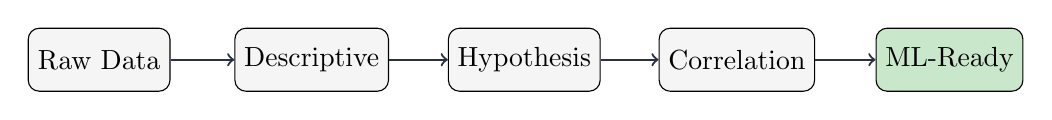
\begin{tikzpicture}[node distance=1.5cm, auto]
            \node[draw, rounded corners, fill=databricksLightGray, minimum width=1.8cm, minimum height=0.8cm] (raw) {Raw Data};
            \node[draw, rounded corners, fill=databricksLightGray, minimum width=1.8cm, minimum height=0.8cm, right of=raw, xshift=1.2cm] (desc) {Descriptive};
            \node[draw, rounded corners, fill=databricksLightGray, minimum width=1.8cm, minimum height=0.8cm, right of=desc, xshift=1.2cm] (hypo) {Hypothesis};
            \node[draw, rounded corners, fill=databricksLightGray, minimum width=1.8cm, minimum height=0.8cm, right of=hypo, xshift=1.2cm] (corr) {Correlation};
            \node[draw, rounded corners, fill=databricksGreen!30, minimum width=1.8cm, minimum height=0.8cm, right of=corr, xshift=1.2cm] (ml) {ML-Ready};
            \draw[->, thick, color=databricksBlue] (raw) -- (desc);
            \draw[->, thick, color=databricksBlue] (desc) -- (hypo);
            \draw[->, thick, color=databricksBlue] (hypo) -- (corr);
            \draw[->, thick, color=databricksBlue] (corr) -- (ml);
        \end{tikzpicture}
    \end{center}
\end{frame}

% ============================================================
% DESCRIPTIVE STATISTICS
% ============================================================
{
\setbeamercolor{background canvas}{bg=databricksBlue}
\begin{frame}[plain]
    \begin{center}
        \vspace{3cm}
        {\Huge\textcolor{databricksWhite}{\textbf{1. Descriptive Statistics}}}\\[0.5cm]
        {\large\textcolor{databricksYellow}{Understanding Your Data}}
    \end{center}
\end{frame}
}

\begin{frame}{Measures of Central Tendency}
    \begin{columns}[T]
        \begin{column}{0.5\textwidth}
            \textcolor{databricksBlue}{\textbf{Mean (Arithmetic Average)}}
            \[
                \bar{x} = \frac{1}{n} \sum_{i=1}^{n} x_i
            \]
            \vspace{0.3cm}
            \textcolor{databricksBlue}{\textbf{Median}}
            \begin{itemize}
                \item Middle value when data is sorted
                \item Robust to outliers
            \end{itemize}
            \vspace{0.3cm}
            \textcolor{databricksBlue}{\textbf{Mode}}
            \begin{itemize}
                \item Most frequently occurring value
            \end{itemize}
        \end{column}
        \begin{column}{0.5\textwidth}
            \begin{block}{When to Use Each}
                \small
                \begin{tabular}{@{}lll@{}}
                    \toprule
                    \textbf{Measure} & \textbf{Best For} & \textbf{Outliers} \\
                    \midrule
                    Mean & Normal dist. & Sensitive \\
                    Median & Skewed data & Robust \\
                    Mode & Categorical & Robust \\
                    \bottomrule
                \end{tabular}
            \end{block}
        \end{column}
    \end{columns}
\end{frame}

\begin{frame}{Measures of Dispersion}
    \begin{columns}[T]
        \begin{column}{0.5\textwidth}
            \textcolor{databricksBlue}{\textbf{Variance}}
            \[
                s^2 = \frac{1}{n-1} \sum_{i=1}^{n} (x_i - \bar{x})^2
            \]
            \vspace{0.2cm}
            \textcolor{databricksBlue}{\textbf{Standard Deviation}}
            \[
                s = \sqrt{s^2}
            \]
            \vspace{0.2cm}
            \textcolor{databricksBlue}{\textbf{IQR (Interquartile Range)}}
            \[
                IQR = Q3 - Q1
            \]
        \end{column}
        \begin{column}{0.5\textwidth}
            \textcolor{databricksBlue}{\textbf{Skewness}}
            \begin{itemize}
                \item \textcolor{databricksRed}{$> 0$}: Right-skewed
                \item \textcolor{databricksGreen}{$= 0$}: Symmetric
                \item \textcolor{databricksRed}{$< 0$}: Left-skewed
            \end{itemize}
            \vspace{0.3cm}
            \textcolor{databricksBlue}{\textbf{Kurtosis}}
            \begin{itemize}
                \item \textcolor{databricksRed}{$> 0$}: Heavy tails
                \item \textcolor{databricksGreen}{$= 0$}: Normal-like
                \item \textcolor{databricksRed}{$< 0$}: Light tails
            \end{itemize}
        \end{column}
    \end{columns}
\end{frame}

\begin{frame}[fragile]{Descriptive Statistics in PySpark}
\begin{lstlisting}
from pyspark.sql import functions as F

# Basic descriptive statistics
events.describe(["price"]).show()

# Extended statistics with percentiles
events.select(
    F.count("price").alias("count"),
    F.mean("price").alias("mean"),
    F.stddev("price").alias("std_dev"),
    F.expr("percentile_approx(price, 0.25)").alias("Q1"),
    F.expr("percentile_approx(price, 0.50)").alias("median"),
    F.expr("percentile_approx(price, 0.75)").alias("Q3"),
    F.skewness("price").alias("skewness"),
    F.kurtosis("price").alias("kurtosis")
).show()

# Detect outliers using IQR method
lower_bound = Q1 - 1.5 * iqr
upper_bound = Q3 + 1.5 * iqr
\end{lstlisting}
\end{frame}

% ============================================================
% HYPOTHESIS TESTING
% ============================================================
{
\setbeamercolor{background canvas}{bg=databricksBlue}
\begin{frame}[plain]
    \begin{center}
        \vspace{3cm}
        {\Huge\textcolor{databricksWhite}{\textbf{2. Hypothesis Testing}}}\\[0.5cm]
        {\large\textcolor{databricksYellow}{Making Data-Driven Decisions}}
    \end{center}
\end{frame}
}

\begin{frame}{Understanding Hypothesis Testing}
    \begin{block}{Key Question}
        \textit{Is the observed pattern in the sample likely to exist in the population, or is it just due to random sampling variation?}
    \end{block}
    \vspace{0.3cm}
    \begin{center}
        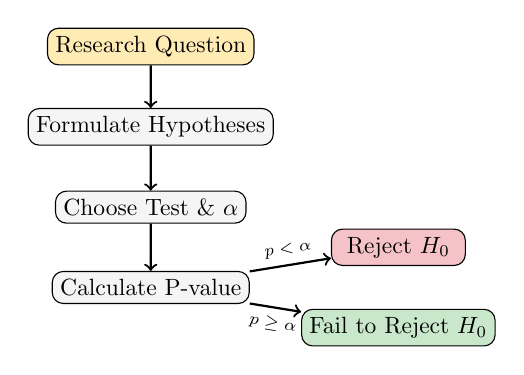
\begin{tikzpicture}[node distance=1.2cm, auto, scale=0.85, transform shape]
            \node[draw, rounded corners, fill=databricksYellow!30, minimum width=2cm] (q) {Research Question};
            \node[draw, rounded corners, fill=databricksLightGray, minimum width=2cm, below of=q] (h) {Formulate Hypotheses};
            \node[draw, rounded corners, fill=databricksLightGray, minimum width=2cm, below of=h] (t) {Choose Test \& $\alpha$};
            \node[draw, rounded corners, fill=databricksLightGray, minimum width=2cm, below of=t] (c) {Calculate P-value};
            \node[draw, rounded corners, fill=databricksRed!30, minimum width=2cm, right of=c, xshift=2.5cm, yshift=0.6cm] (r) {Reject $H_0$};
            \node[draw, rounded corners, fill=databricksGreen!30, minimum width=2cm, right of=c, xshift=2.5cm, yshift=-0.6cm] (f) {Fail to Reject $H_0$};
            \draw[->, thick] (q) -- (h);
            \draw[->, thick] (h) -- (t);
            \draw[->, thick] (t) -- (c);
            \draw[->, thick] (c) -- node[above, sloped, font=\scriptsize] {$p < \alpha$} (r);
            \draw[->, thick] (c) -- node[below, sloped, font=\scriptsize] {$p \geq \alpha$} (f);
        \end{tikzpicture}
    \end{center}
\end{frame}

\begin{frame}{Types of Hypotheses}
    \begin{columns}[T]
        \begin{column}{0.5\textwidth}
            \textcolor{databricksBlue}{\textbf{Null Hypothesis ($H_0$)}}
            \begin{itemize}
                \item Default assumption
                \item No effect/difference
                \item Status quo
            \end{itemize}
            \vspace{0.3cm}
            \textcolor{databricksRed}{\textbf{Alternative Hypothesis ($H_1$)}}
            \begin{itemize}
                \item What we're testing for
                \item Contradicts $H_0$
            \end{itemize}
        \end{column}
        \begin{column}{0.5\textwidth}
            \begin{block}{Test Types}
                \small
                \begin{tabular}{@{}ll@{}}
                    \toprule
                    \textbf{Type} & \textbf{Alternative} \\
                    \midrule
                    Two-tailed & $\mu \neq \mu_0$ \\
                    Left-tailed & $\mu < \mu_0$ \\
                    Right-tailed & $\mu > \mu_0$ \\
                    \bottomrule
                \end{tabular}
            \end{block}
        \end{column}
    \end{columns}
\end{frame}

\begin{frame}{P-Value and Significance Level}
    \begin{columns}[T]
        \begin{column}{0.5\textwidth}
            \textcolor{databricksBlue}{\textbf{Significance Level ($\alpha$)}}
            \begin{itemize}
                \item $\alpha = 0.05$ (5\%): Most common
                \item $\alpha = 0.01$ (1\%): More stringent
                \item $\alpha = 0.10$ (10\%): Exploratory
            \end{itemize}
            \vspace{0.3cm}
            \textcolor{databricksBlue}{\textbf{P-Value}}
            \[
                P(\text{Observed} | H_0 \text{ is true})
            \]
        \end{column}
        \begin{column}{0.5\textwidth}
            \begin{alertblock}{Decision Rule}
                \begin{itemize}
                    \item \textcolor{databricksRed}{$p < \alpha$}: Reject $H_0$
                    \item \textcolor{databricksGreen}{$p \geq \alpha$}: Fail to reject $H_0$
                \end{itemize}
            \end{alertblock}
            \vspace{0.3cm}
            \textcolor{databricksBlue}{\textbf{Example:}}\\
            If $p = 0.03$ and $\alpha = 0.05$:\\
            $\rightarrow$ Reject $H_0$ (significant)
        \end{column}
    \end{columns}
\end{frame}

\begin{frame}{Types of Errors}
    \begin{center}
        \begin{tabular}{@{}l|cc@{}}
            \toprule
            \textbf{Decision} & \textbf{$H_0$ True} & \textbf{$H_0$ False} \\
            \midrule
            Reject $H_0$ & \textcolor{databricksRed}{\textbf{Type I ($\alpha$)}} & \textcolor{databricksGreen}{\checkmark Correct} \\
            & False Positive & (Power) \\
            \midrule
            Fail to Reject & \textcolor{databricksGreen}{\checkmark Correct} & \textcolor{databricksRed}{\textbf{Type II ($\beta$)}} \\
            & & False Negative \\
            \bottomrule
        \end{tabular}
    \end{center}
    \vspace{0.5cm}
    \begin{columns}[T]
        \begin{column}{0.5\textwidth}
            \textcolor{databricksBlue}{\textbf{Statistical Power}}
            \[
                \text{Power} = 1 - \beta
            \]
        \end{column}
        \begin{column}{0.5\textwidth}
            \textcolor{databricksBlue}{\textbf{Factors Affecting Power:}}
            \begin{itemize}
                \item Sample size $\uparrow$
                \item Effect size $\uparrow$
                \item Variance $\downarrow$
            \end{itemize}
        \end{column}
    \end{columns}
\end{frame}

\begin{frame}{Common Statistical Tests}
    \begin{columns}[T]
        \begin{column}{0.5\textwidth}
            \textcolor{databricksBlue}{\textbf{Z-Test}}
            \[
                z = \frac{\bar{x} - \mu_0}{\sigma / \sqrt{n}}
            \]
            \begin{itemize}
                \item Known population $\sigma$
                \item Large sample ($n > 30$)
            \end{itemize}
            \vspace{0.3cm}
            \textcolor{databricksBlue}{\textbf{T-Test}}
            \[
                t = \frac{\bar{x} - \mu_0}{s / \sqrt{n}}
            \]
            \begin{itemize}
                \item Unknown population $\sigma$
            \end{itemize}
        \end{column}
        \begin{column}{0.5\textwidth}
            \textcolor{databricksBlue}{\textbf{Chi-Square Test}}
            \[
                \chi^2 = \sum \frac{(O_i - E_i)^2}{E_i}
            \]
            \begin{itemize}
                \item Categorical data
                \item Independence tests
            \end{itemize}
            \vspace{0.3cm}
            \textcolor{databricksBlue}{\textbf{Two-Sample T-Test}}
            \[
                t = \frac{\bar{x}_1 - \bar{x}_2}{\sqrt{\frac{s_1^2}{n_1} + \frac{s_2^2}{n_2}}}
            \]
        \end{column}
    \end{columns}
\end{frame}

% ============================================================
% A/B TESTING
% ============================================================
{
\setbeamercolor{background canvas}{bg=databricksBlue}
\begin{frame}[plain]
    \begin{center}
        \vspace{3cm}
        {\Huge\textcolor{databricksWhite}{\textbf{3. A/B Test Design}}}\\[0.5cm]
        {\large\textcolor{databricksYellow}{Controlled Experiments}}
    \end{center}
\end{frame}
}

\begin{frame}{What is A/B Testing?}
    \begin{block}{Definition}
        A controlled experiment comparing two or more variants to determine which performs better.
    \end{block}
    \vspace{0.3cm}
    \begin{center}
        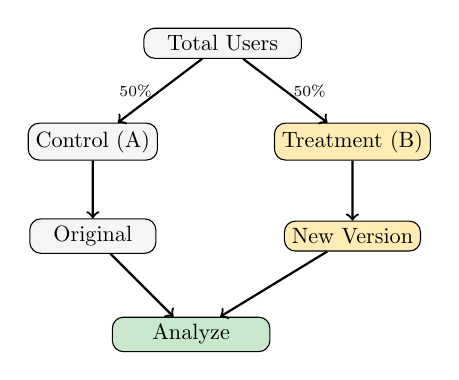
\begin{tikzpicture}[node distance=1.5cm, scale=0.8, transform shape]
            \node[draw, rounded corners, fill=databricksLightGray, minimum width=2.5cm] (pop) {Total Users};
            \node[draw, rounded corners, fill=databricksLightGray, minimum width=2cm, below left of=pop, xshift=-1cm, yshift=-0.5cm] (ctrl) {Control (A)};
            \node[draw, rounded corners, fill=databricksYellow!30, minimum width=2cm, below right of=pop, xshift=1cm, yshift=-0.5cm] (treat) {Treatment (B)};
            \node[draw, rounded corners, fill=databricksLightGray, minimum width=2cm, below of=ctrl] (orig) {Original};
            \node[draw, rounded corners, fill=databricksYellow!30, minimum width=2cm, below of=treat] (new) {New Version};
            \node[draw, rounded corners, fill=databricksGreen!30, minimum width=2.5cm, below right of=orig, xshift=0.5cm, yshift=-0.5cm] (analyze) {Analyze};
            \draw[->, thick] (pop) -- node[left, font=\scriptsize] {50\%} (ctrl);
            \draw[->, thick] (pop) -- node[right, font=\scriptsize] {50\%} (treat);
            \draw[->, thick] (ctrl) -- (orig);
            \draw[->, thick] (treat) -- (new);
            \draw[->, thick] (orig) -- (analyze);
            \draw[->, thick] (new) -- (analyze);
        \end{tikzpicture}
    \end{center}
\end{frame}

\begin{frame}{Key Metrics \& Parameters}
    \begin{columns}[T]
        \begin{column}{0.5\textwidth}
            \textcolor{databricksBlue}{\textbf{Metric Types}}
            \begin{itemize}
                \item \textcolor{databricksRed}{$\triangleright$} \textbf{Primary:} Main success indicator
                \item \textcolor{databricksRed}{$\triangleright$} \textbf{Secondary:} Supporting metrics
                \item \textcolor{databricksRed}{$\triangleright$} \textbf{Guardrail:} Must not worsen
            \end{itemize}
        \end{column}
        \begin{column}{0.5\textwidth}
            \textcolor{databricksBlue}{\textbf{Key Parameters}}
            \begin{itemize}
                \item \textcolor{databricksRed}{$\triangleright$} Baseline rate ($p_0$)
                \item \textcolor{databricksRed}{$\triangleright$} MDE (Min. Detectable Effect)
                \item \textcolor{databricksRed}{$\triangleright$} Significance ($\alpha$): 0.05
                \item \textcolor{databricksRed}{$\triangleright$} Power ($1-\beta$): 0.80
            \end{itemize}
        \end{column}
    \end{columns}
\end{frame}

\begin{frame}{Sample Size Calculation}
    \textcolor{databricksBlue}{\textbf{Formula for Two-Proportion Z-Test:}}
    \[
        n = \frac{2 \cdot (Z_{\alpha/2} + Z_{\beta})^2 \cdot \bar{p}(1-\bar{p})}{(p_1 - p_0)^2}
    \]
    \vspace{0.3cm}
    \begin{exampleblock}{Example Calculation}
        \small
        Given: $p_0 = 0.10$, MDE = 0.02, $\alpha = 0.05$, Power = 0.80
        \begin{itemize}
            \item $\bar{p} = \frac{0.10 + 0.12}{2} = 0.11$
            \item $n = \frac{2 \times (1.96 + 0.84)^2 \times 0.11 \times 0.89}{0.0004} \approx 3,838$ per group
        \end{itemize}
        \textbf{Total: $\sim$7,676 users needed}
    \end{exampleblock}
\end{frame}

\begin{frame}{Common Pitfalls}
    \begin{center}
        \begin{tabular}{@{}lll@{}}
            \toprule
            \textbf{Pitfall} & \textbf{Problem} & \textbf{Solution} \\
            \midrule
            Peeking & Inflated false positives & Pre-commit to duration \\
            Multiple tests & Increased Type I errors & Bonferroni correction \\
            Simpson's Paradox & Misleading aggregates & Segment analysis \\
            Novelty effect & Temporary engagement & Run longer \\
            \bottomrule
        \end{tabular}
    \end{center}
\end{frame}

% ============================================================
% CORRELATION ANALYSIS
% ============================================================
{
\setbeamercolor{background canvas}{bg=databricksBlue}
\begin{frame}[plain]
    \begin{center}
        \vspace{3cm}
        {\Huge\textcolor{databricksWhite}{\textbf{4. Correlation Analysis}}}\\[0.5cm]
        {\large\textcolor{databricksYellow}{Measuring Relationships}}
    \end{center}
\end{frame}
}

\begin{frame}{Types of Correlation}
    \begin{columns}[T]
        \begin{column}{0.33\textwidth}
            \begin{center}
                \textcolor{databricksGreen}{\textbf{Positive}}\\
                $r > 0$\\[0.5cm]
                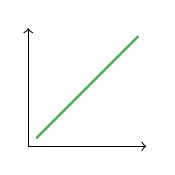
\begin{tikzpicture}[scale=0.5]
                    \draw[->] (0,0) -- (3,0);
                    \draw[->] (0,0) -- (0,3);
                    \draw[thick, databricksGreen] (0.2,0.2) -- (2.8,2.8);
                \end{tikzpicture}\\
                X $\uparrow$ $\Rightarrow$ Y $\uparrow$
            \end{center}
        \end{column}
        \begin{column}{0.33\textwidth}
            \begin{center}
                \textcolor{databricksRed}{\textbf{Negative}}\\
                $r < 0$\\[0.5cm]
                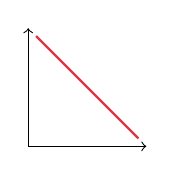
\begin{tikzpicture}[scale=0.5]
                    \draw[->] (0,0) -- (3,0);
                    \draw[->] (0,0) -- (0,3);
                    \draw[thick, databricksRed] (0.2,2.8) -- (2.8,0.2);
                \end{tikzpicture}\\
                X $\uparrow$ $\Rightarrow$ Y $\downarrow$
            \end{center}
        \end{column}
        \begin{column}{0.33\textwidth}
            \begin{center}
                \textcolor{databricksGray}{\textbf{No Correlation}}\\
                $r \approx 0$\\[0.5cm]
                \begin{tikzpicture}[scale=0.5]
                    \draw[->] (0,0) -- (3,0);
                    \draw[->] (0,0) -- (0,3);
                    \draw[thick, databricksGray, dashed] (0.5,1.5) -- (2.5,1.5);
                \end{tikzpicture}\\
                No linear relation
            \end{center}
        \end{column}
    \end{columns}
\end{frame}

\begin{frame}{Pearson Correlation Coefficient}
    \textcolor{databricksBlue}{\textbf{Formula:}}
    \[
        r = \frac{\sum_{i=1}^{n}(x_i - \bar{x})(y_i - \bar{y})}{\sqrt{\sum(x_i - \bar{x})^2} \cdot \sqrt{\sum(y_i - \bar{y})^2}}
    \]
    \vspace{0.3cm}
    \begin{center}
        \begin{tabular}{@{}ll@{}}
            \toprule
            \textbf{r Value} & \textbf{Interpretation} \\
            \midrule
            0.90 -- 1.00 & Very strong \\
            0.70 -- 0.89 & Strong \\
            0.50 -- 0.69 & Moderate \\
            0.30 -- 0.49 & Weak \\
            0.00 -- 0.29 & Very weak \\
            \bottomrule
        \end{tabular}
    \end{center}
    \vspace{0.3cm}
    \textcolor{databricksBlue}{\textbf{Coefficient of Determination:}} $r^2$ = variance explained
\end{frame}

\begin{frame}[fragile]{Correlation in PySpark}
\begin{lstlisting}
from pyspark.ml.stat import Correlation
from pyspark.ml.feature import VectorAssembler

# Method 1: Two columns
correlation = events.stat.corr("price", "conversion_rate")

# Method 2: Correlation matrix
numeric_columns = ["price", "quantity", "discount", "revenue"]

assembler = VectorAssembler(inputCols=numeric_columns, outputCol="features")
vector_df = assembler.transform(events.na.drop(subset=numeric_columns))

correlation_matrix = Correlation.corr(vector_df, "features", "pearson").head()
corr_array = correlation_matrix[0].toArray()

# Print correlation matrix
for i, col in enumerate(numeric_columns):
    print(f"{col}", end=" ")
    for j in range(len(numeric_columns)):
        print(f"{corr_array[i][j]:.3f}", end=" ")
\end{lstlisting}
\end{frame}

% ============================================================
% FEATURE ENGINEERING
% ============================================================
{
\setbeamercolor{background canvas}{bg=databricksBlue}
\begin{frame}[plain]
    \begin{center}
        \vspace{3cm}
        {\Huge\textcolor{databricksWhite}{\textbf{5. Feature Engineering}}}\\[0.5cm]
        {\large\textcolor{databricksYellow}{Transforming Raw Data for ML}}
    \end{center}
\end{frame}
}

\begin{frame}{Types of Feature Engineering}
    \begin{center}
        \small
        \begin{tabular}{@{}llp{5cm}@{}}
            \toprule
            \textbf{Type} & \textbf{Description} & \textbf{Examples} \\
            \midrule
            \textcolor{databricksBlue}{\textbf{Temporal}} & Time-based patterns & Hour, day of week, season \\
            \textcolor{databricksBlue}{\textbf{Aggregation}} & Summarize data & Total purchases, avg order \\
            \textcolor{databricksBlue}{\textbf{Transformation}} & Change distribution & Log, power, binning \\
            \textcolor{databricksBlue}{\textbf{Interaction}} & Combine features & Price $\times$ Quantity, ratios \\
            \textcolor{databricksBlue}{\textbf{Window}} & Rolling metrics & Moving avg, cumulative \\
            \textcolor{databricksBlue}{\textbf{Encoding}} & Categorical to numeric & One-hot, label encoding \\
            \bottomrule
        \end{tabular}
    \end{center}
\end{frame}

\begin{frame}{Numerical Transformations}
    \begin{columns}[T]
        \begin{column}{0.5\textwidth}
            \textcolor{databricksBlue}{\textbf{Log Transformation}}
            \[
                x' = \log(x + 1)
            \]
            \begin{itemize}
                \item Handles skewed distributions
                \item Reduces outlier impact
            \end{itemize}
            \vspace{0.3cm}
            \textcolor{databricksBlue}{\textbf{Standardization (Z-score)}}
            \[
                z = \frac{x - \mu}{\sigma}
            \]
        \end{column}
        \begin{column}{0.5\textwidth}
            \textcolor{databricksBlue}{\textbf{Min-Max Scaling}}
            \[
                x' = \frac{x - x_{min}}{x_{max} - x_{min}}
            \]
            \begin{itemize}
                \item Scales to [0, 1] range
            \end{itemize}
            \vspace{0.3cm}
            \textcolor{databricksBlue}{\textbf{Square Root}}
            \[
                x' = \sqrt{x}
            \]
        \end{column}
    \end{columns}
\end{frame}

\begin{frame}[fragile]{Feature Engineering in PySpark}
\begin{lstlisting}
from pyspark.sql import functions as F
from pyspark.sql.window import Window

# Temporal features
features = events.withColumn("hour", F.hour("event_time")) \
    .withColumn("day_of_week", F.dayofweek("event_date")) \
    .withColumn("is_weekend", F.dayofweek("event_date").isin([1, 7]).cast("int"))

# Log transformation
features = features.withColumn("price_log", F.log(F.col("price") + 1))

# Window features
user_window = Window.partitionBy("user_id").orderBy("event_time")
features = features.withColumn("event_sequence", F.row_number().over(user_window))

# Aggregation features
user_agg = events.groupBy("user_id").agg(
    F.count("*").alias("total_events"),
    F.avg("price").alias("avg_price"),
    F.sum(F.when(F.col("event_type") == "purchase", 1).otherwise(0)).alias("purchases")
)
\end{lstlisting}
\end{frame}

\begin{frame}{Window Function Templates}
    \textcolor{databricksBlue}{\textbf{Common Window Patterns:}}
    \vspace{0.3cm}
    \begin{center}
        \small
        \begin{tabular}{@{}lp{6cm}@{}}
            \toprule
            \textbf{Pattern} & \textbf{Use Case} \\
            \midrule
            \texttt{partitionBy().orderBy()} & Basic ordering within groups \\
            \texttt{rowsBetween(-4, 0)} & Last 5 rows (rolling) \\
            \texttt{unboundedPreceding, currentRow} & Cumulative calculations \\
            \texttt{rangeBetween(-86400, 0)} & Last 24 hours (time-based) \\
            \bottomrule
        \end{tabular}
    \end{center}
    \vspace{0.3cm}
    \textcolor{databricksBlue}{\textbf{Common Functions:}}
    \begin{itemize}
        \item \texttt{row\_number()}, \texttt{rank()}, \texttt{lag()}, \texttt{lead()}
        \item \texttt{sum()}, \texttt{avg()}, \texttt{first()}, \texttt{last()}
    \end{itemize}
\end{frame}

% ============================================================
% BEST PRACTICES
% ============================================================
{
\setbeamercolor{background canvas}{bg=databricksBlue}
\begin{frame}[plain]
    \begin{center}
        \vspace{3cm}
        {\Huge\textcolor{databricksWhite}{\textbf{6. Best Practices}}}\\[0.5cm]
        {\large\textcolor{databricksYellow}{\& Quick Reference}}
    \end{center}
\end{frame}
}

\begin{frame}{Statistical Analysis Best Practices}
    \begin{itemize}
        \item \textcolor{databricksBlue}{\textbf{Check Assumptions:}} Verify normality before parametric tests
        \item \textcolor{databricksBlue}{\textbf{Use Appropriate Tests:}} Match test to data type
        \item \textcolor{databricksBlue}{\textbf{Multiple Testing Correction:}} Apply Bonferroni or FDR
        \item \textcolor{databricksBlue}{\textbf{Report Effect Size:}} Not just p-values
        \item \textcolor{databricksBlue}{\textbf{Confidence Intervals:}} Always include them
        \item \textcolor{databricksBlue}{\textbf{Sample Size:}} Ensure adequacy before testing
    \end{itemize}
\end{frame}

\begin{frame}{Feature Engineering Best Practices}
    \begin{itemize}
        \item \textcolor{databricksBlue}{\textbf{Domain Knowledge:}} Create meaningful features
        \item \textcolor{databricksBlue}{\textbf{Avoid Data Leakage:}} No future information
        \item \textcolor{databricksBlue}{\textbf{Handle Missing Values:}} Impute appropriately
        \item \textcolor{databricksBlue}{\textbf{Scale Features:}} Normalize for sensitive algorithms
        \item \textcolor{databricksBlue}{\textbf{Remove Redundancy:}} Drop correlated features
        \item \textcolor{databricksBlue}{\textbf{Validate Transformations:}} Check distributions
    \end{itemize}
    \vspace{0.5cm}
    \begin{alertblock}{Common Pitfalls}
        \begin{itemize}
            \item Data leakage using test data in training
            \item Overfitting with too many features
            \item Ignoring time order in temporal data
        \end{itemize}
    \end{alertblock}
\end{frame}

\begin{frame}{Quick Reference: Key Formulas}
    \begin{center}
        \small
        \begin{tabular}{@{}ll@{}}
            \toprule
            \textbf{Metric} & \textbf{Formula} \\
            \midrule
            Mean & $\bar{x} = \frac{\sum x_i}{n}$ \\[0.3cm]
            Variance & $s^2 = \frac{\sum(x_i - \bar{x})^2}{n-1}$ \\[0.3cm]
            Pearson Correlation & $r = \frac{\text{Cov}(X,Y)}{\sigma_X \cdot \sigma_Y}$ \\[0.3cm]
            Z-Score & $z = \frac{x - \mu}{\sigma}$ \\[0.3cm]
            T-Statistic & $t = \frac{\bar{x} - \mu_0}{s/\sqrt{n}}$ \\[0.3cm]
            A/B Sample Size & $n = \frac{2(Z_{\alpha/2} + Z_\beta)^2 \bar{p}(1-\bar{p})}{(p_1-p_0)^2}$ \\
            \bottomrule
        \end{tabular}
    \end{center}
\end{frame}

\begin{frame}{PySpark Statistical Functions}
    \begin{center}
        \small
        \begin{tabular}{@{}llp{4.5cm}@{}}
            \toprule
            \textbf{Function} & \textbf{Description} & \textbf{Example} \\
            \midrule
            \texttt{F.mean()} & Average & \texttt{df.select(F.mean("col"))} \\
            \texttt{F.stddev()} & Std deviation & \texttt{df.select(F.stddev("col"))} \\
            \texttt{F.variance()} & Variance & \texttt{df.select(F.variance("col"))} \\
            \texttt{F.skewness()} & Skewness & \texttt{df.select(F.skewness("col"))} \\
            \texttt{F.kurtosis()} & Kurtosis & \texttt{df.select(F.kurtosis("col"))} \\
            \texttt{stat.corr()} & Correlation & \texttt{df.stat.corr("col1", "col2")} \\
            \texttt{describe()} & Summary & \texttt{df.describe(["col"])} \\
            \bottomrule
        \end{tabular}
    \end{center}
\end{frame}

% ============================================================
% RESOURCES
% ============================================================
\begin{frame}{Resources}
    \begin{itemize}
        \item \textcolor{databricksBlue}{\textbf{Apache Spark ML Guide}}\\
              \url{https://spark.apache.org/docs/latest/ml-guide.html}
        \item \textcolor{databricksBlue}{\textbf{Databricks Documentation}}\\
              \url{https://docs.databricks.com/}
        \item \textcolor{databricksBlue}{\textbf{Spark by Examples}}\\
              \url{https://sparkbyexamples.com/}
        \item \textcolor{databricksBlue}{\textbf{Databricks ML Lifecycle}}\\
              \url{https://docs.databricks.com/machine-learning/index.html}
        \item \textcolor{databricksBlue}{\textbf{A/B Testing Guide}}\\
              \url{https://www.optimizely.com/optimization-glossary/ab-testing/}
    \end{itemize}
\end{frame}

% ============================================================
% THANK YOU
% ============================================================
{
\setbeamercolor{background canvas}{bg=databricksBlue}
\begin{frame}[plain]
    \begin{center}
        \vspace{2cm}
        {\Huge\textcolor{databricksWhite}{\textbf{Thank You!}}}\\[1cm]
        {\Large\textcolor{databricksYellow}{Day 11 Complete}}\\[0.5cm]
        {\normalsize\textcolor{databricksWhite}{Statistical Analysis \& ML Preparation}}\\[1.5cm]
        {\small\textcolor{databricksLightGray}{
            \href{https://easy-ai-labs.lovable.app/}{Easy AI Labs} | 
            \href{https://www.linkedin.com/in/yashkavaiya}{Yash Kavaiya} | 
            \href{https://www.linkedin.com/company/genai-guru}{Gen AI Guru}
        }}
    \end{center}
\end{frame}
}

\end{document}
